\chapter{Getting Started} \label{ch:gettingStarted}

\section{Installation} \label{sec:installation}

\vvase{} does not include any installation process or changes to the machine registry.  Simply place the executable and the pdf manual into the same directory.  After running the first time, any changes to the default settings are saved to a configuration file which will appear in the directory from which the application is run.

\section{Overview} \label{sec:overview}

Upon starting \vvase{} for the first time, the screen will look like Fig.~\ref{fig:defaultStartup}.  

\begin{figure}
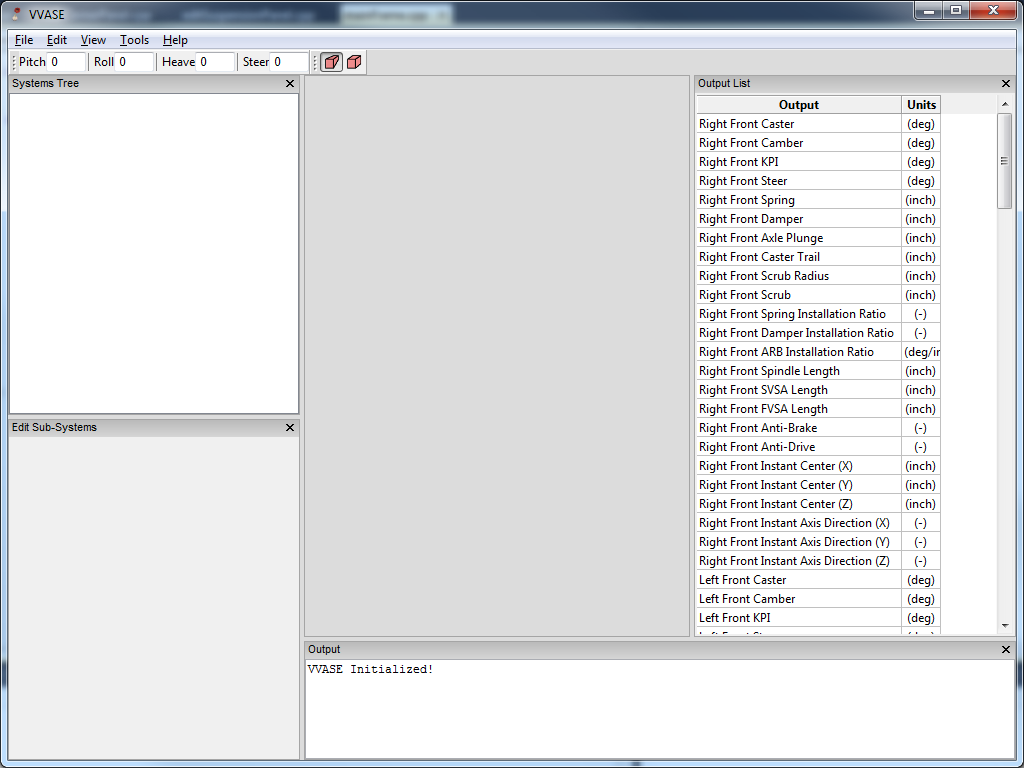
\includegraphics[width=\textwidth]{images/defaultStartup} \label{fig:defaultStartup}
\caption{Default screen configuration}
\centering
\end{figure}

\subsection{Systems Tree} \label{ssec:systemsTree}
\subsection{Edit Panel} \label{ssec:editPanel}
\subsection{Output List} \label{ssec:outputList}
\subsection{Output Pane} \label{ssec:outputPane}
\subsection{Main Display Area} \label{ssec:mainDisplayArea}
\subsection{Kinematics Toolbar} \label{ssec:kinematicsToolbar}
\subsection{3D Toolbar} \label{ssec:3DToolbar}

\section{Options} \label{sec:options}

\begin{figure}
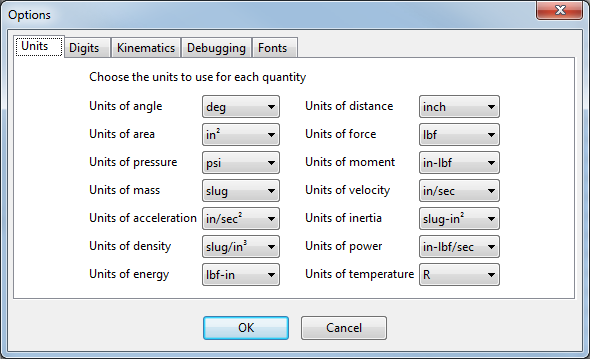
\includegraphics[width=\textwidth]{images/optionsUnits} \label{fig:optionsUnits}
\caption{Units options}
\centering
\end{figure}

\begin{figure}
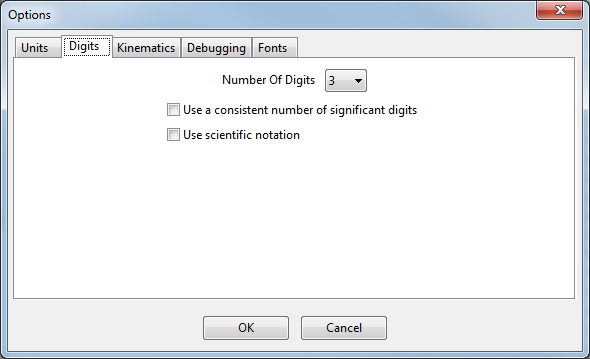
\includegraphics[width=\textwidth]{images/optionsDigits} \label{fig:optionsDigits}
\caption{Digits options}
\centering
\end{figure}

\begin{figure}
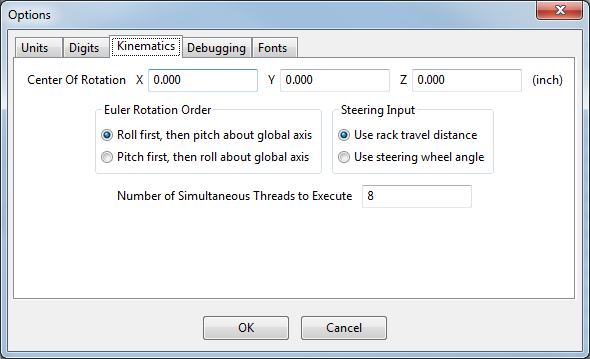
\includegraphics[width=\textwidth]{images/optionsKinematics} \label{fig:optionsKinematics}
\caption{Kinematics options}
\centering
\end{figure}

\begin{figure}
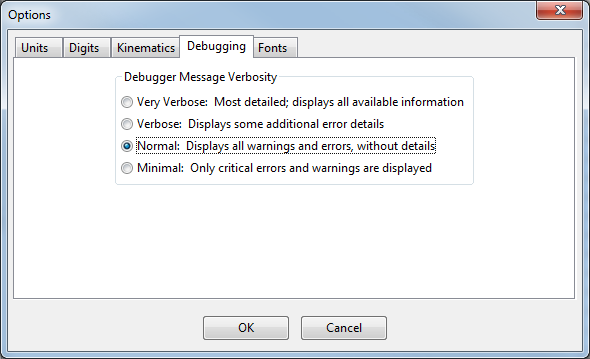
\includegraphics[width=\textwidth]{images/optionsDebugging} \label{fig:optionsDebugging}
\caption{Debugging options}
\centering
\end{figure}

\begin{figure}
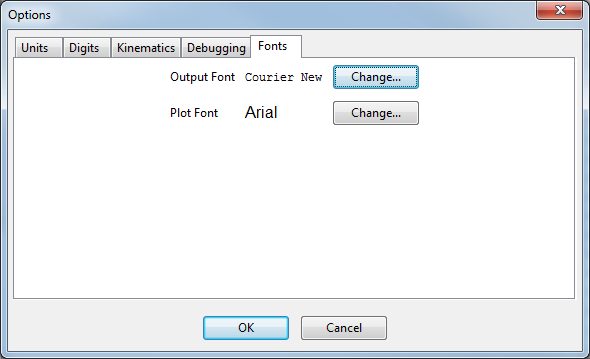
\includegraphics[width=\textwidth]{images/optionsFonts} \label{fig:optionsFonts}
\caption{Fonts options}
\centering
\end{figure}